\documentclass{ieeeaccess}
\usepackage{cite}
\usepackage{amsmath,amssymb,amsfonts}
\usepackage{algorithmic}
\usepackage{graphicx}
\usepackage{textcomp}
\usepackage{booktabs}

\def\BibTeX{{\rm B\kern-.05em{\sc i\kern-.025em b}\kern-.08em
    T\kern-.1667em\lower.7ex\hbox{E}\kern-.125emX}}

\begin{document}
\history{Date of publication xxxx 00, 0000, date of current version xxxx 00, 0000.}
\doi{10.1109/ACCESS.2026.DOI}

\title{Information-Theoretic Adaptive Differential Privacy and Authenticated Cryptographic Transport in Decentralized Federated Learning: Bounding Gradient Reconstruction in Non-IID Breast Cancer Histopathology}

\author{\uppercase{Mateo Francisco O\~nate Escobar}\authorrefmark{1}, (ORCID: 0009-0000-0000-0001), and \uppercase{Demian Viteri}\authorrefmark{2}, (ORCID: 0009-0000-0000-0002)}
\address[1]{School of Mathematical and Computational Sciences, Yachay Tech University, Urcuqu\'i 100119, Ecuador (e-mail: mateo.onate@yachaytech.edu.ec)}
\address[2]{School of Mathematical and Computational Sciences, Yachay Tech University, Urcuqu\'i 100119, Ecuador (e-mail: demian.viteri@yachaytech.edu.ec)}

\corresp{Corresponding author: Mateo Francisco O\~nate Escobar (e-mail: mateo.onate@yachaytech.edu.ec).}

\begin{abstract}
Decentralized federated learning (FL) enables medical institutions to collaboratively train diagnostic models without pooling raw patient biopsies, yet peer-to-peer (P2P) parameter exchanges remain exposed to man-in-the-middle (MitM) interception, gradient inversion, and multi-round membership inference attacks. Standard differential privacy (DP) with static clipping and uniform Gaussian perturbation degrades minority tumor features under non-IID institutional domain shifts and leaves unencrypted updates vulnerable in transit. We propose an adaptive DP and authenticated cryptographic P2P protocol implemented over the decentralized NEBULA framework. At the statistical layer, each hospital enforces per-example $L_2$ gradient clipping via a decaying threshold $C_t$ and injects Gaussian noise $\sigma_t$ calibrated via a held-out public variance proxy $\widehat{\text{Var}}_{t-1}$, tracked under Poisson subsampling via R\'enyi Differential Privacy (RDP). At the cryptographic transport layer, nodes establish ephemeral session keys via Elliptic-Curve Diffie-Hellman over Curve25519 (X25519, RFC 7748) with HKDF-SHA256, encrypt gradient payloads via AES-256-CTR (NIST SP 800-38A), and authenticate packets under an Encrypt-then-Sign construction using Ed25519 (RFC 8032) prior to decentralized gossip consensus. Evaluated across five hospital nodes on Camelyon17-WILDS ($96 \times 96 \times 3$ patches) under institutional shift and Dirichlet label skew ($\beta \in \{0.1, 0.5\}$) for privacy budgets $\varepsilon \in \{1.0, 2.0, 3.0\}$ at $\delta = 10^{-5}$, our framework bounds Deep Leakage from Gradients (DLG) and Venom reconstruction structural similarity below $0.055$ (down from $0.9625$ unprotected), maintains membership inference near random guessing ($\text{MIA-AUC} = 0.528$), adds only $103.2\text{ ms}$ cryptographic overhead on $44\text{ MB}$ ResNet-18 payloads, and achieves clinical diagnostic utility of $\text{AUROC} = 0.896 \pm 0.004$ and $91.1\%$ sensitivity at $\varepsilon = 2.0$.
\end{abstract}

\begin{keywords}
Adaptive differential privacy, AES-256-CTR, applied cryptography, breast cancer histopathology, Curve25519, decentralized federated learning, Ed25519, gradient inversion attacks, R\'enyi differential privacy.
\end{keywords}

\titlepgskip=-15pt
\maketitle

\section{INTRODUCTION}
Multi-institutional collaboration is essential for training generalizable deep learning models in computational pathology, and decentralized federated learning (DFL) enables peer-to-peer (P2P) model training across hospitals without centralizing sensitive whole-slide images (WSIs)~\cite{ref1}. Frameworks such as NEBULA orchestrate autonomous medical nodes over decentralized overlays without relying on a central parameter server~\cite{ref1}. However, exchanging model updates instead of raw images does not guarantee privacy: shared gradients remain vulnerable to reconstruction attacks such as Deep Leakage from Gradients (DLG)~\cite{ref2} and cosine/diffusion-guided gradient inversion (Venom)~\cite{ref3}, as well as multi-round membership inference attacks (FedMIA)~\cite{ref4}.

Differential privacy (DP)~\cite{ref5,ref6} provides formal $(\varepsilon, \delta)$-indistinguishability, yet conventional DP-FedAvg applies a static per-example clipping threshold ($C=1.0$) and uniform Gaussian noise across all training rounds. In cross-silo breast cancer lymph node histopathology (Camelyon17-WILDS)~\cite{ref7,ref8}, differences in hematoxylin and eosin (H\&E) staining protocols and scanner hardware induce severe non-IID client drift~\cite{ref9}. Under such heterogeneity, static clipping truncates informative minority-class gradients while uniform perturbation pushes diagnostic performance below clinical acceptability thresholds ($\text{AUROC} < 0.85, \text{sensitivity} < 90\%$)~\cite{ref10}.

Prior work leaves three unresolved gaps: (i) standard aggregators suffer severe utility loss under static DP noise in non-IID medical regimes~\cite{ref10,ref11}; (ii) heuristic adaptive clipping methods~\cite{ref12,ref13,ref14} compute uncalibrated data-dependent statistics or lack tight R\'enyi DP composition bounds against gradient inversion~\cite{ref15,ref16}; and (iii) P2P frameworks transmit perturbed updates over unauthenticated channels without cryptographic confidentiality or integrity verification~\cite{ref17,ref18,ref19}.

\section{CRYPTOGRAPHIC BACKGROUND AND SYSTEM THREAT MODEL}

\subsection{System Architecture and Decentralized Topology}
We consider a peer-to-peer cross-silo deployment over the NEBULA framework~\cite{ref1} comprising $K = 5$ hospital nodes, each holding isolated tissue patches from the Camelyon17-WILDS benchmark~\cite{ref7,ref8}. Nodes communicate directly over a decentralized P2P overlay without any central server.

\subsection{Cryptographic and Privacy Threat Model}
\textbf{Adversary Model.} Consistent with a fully decentralized P2P architecture, we eliminate any central entity assumption. The threat model comprises: (i) an external active Man-in-the-Middle (MitM) network eavesdropper monitoring inter-hospital communication links, and (ii) a semi-honest (honest-but-curious) coalition of up to $K - 1$ colluding peer hospital nodes.

\textbf{Adversary Capabilities.} The external eavesdropper intercepts P2P packets to attempt packet tampering or gradient reconstruction, while colluding peer nodes inspect decrypted peer updates $\tilde{g}_t^k$ during gossip aggregation to execute DLG~\cite{ref2}, Venom proxy inversion~\cite{ref3}, and multi-round likelihood-ratio membership inference (FedMIA)~\cite{ref4}.

\textbf{Security Definition.} A randomized mechanism $\mathcal{M}$ under Poisson subsampling rate $q$~\cite{ref18} satisfies $(\varepsilon, \delta)$-DP if for all neighboring clinical datasets $D, D'$ differing in a single sample and all measurable sets $\mathcal{S}$:
\begin{equation}
\Pr[\mathcal{M}(D) \in \mathcal{S}] \le e^{\varepsilon} \Pr[\mathcal{M}(D') \in \mathcal{S}] + \delta.
\label{eq:dp_def}
\end{equation}

\section{PROPOSED ADAPTIVE PRIVACY AND CRYPTOGRAPHIC METHODOLOGY}

\subsection{Per-Example Dynamic $L_2$-Sensitivity Bounding}
At communication round $t$, hospital node $k$ samples a local mini-batch $B_t^k$ via Poisson subsampling with probability $q$. For each individual histopathology patch $x_i \in B_t^k$, the per-example gradient is computed via vectorized automatic differentiation (\texttt{torch.func.vmap}):
\begin{equation}
g_{t,i}^k = \nabla_w \mathcal{L}(w_t^k; x_i, y_i).
\label{eq:per_example_grad}
\end{equation}
Rather than applying a static threshold $C=1$, we enforce per-example dynamic clipping using a decaying sensitivity bound $C_t$:
\begin{equation}
\bar{g}_{t,i}^k = \frac{g_{t,i}^k}{\max\left(1, \frac{\|g_{t,i}^k\|_2}{C_t}\right)}, \quad C_t = C_0 \exp(-\gamma t) + \lambda \sqrt{\widehat{\text{Var}}_{t-1}} \exp(-\beta_c t),
\label{eq:dynamic_clip}
\end{equation}
where $\widehat{\text{Var}}_{t-1}$ is the normalized gradient norm variance estimated on a held-out $3.5\%$ public calibration reference split, incurring zero privacy cost on patient data.

\subsection{Variance- and Entropy-Calibrated Perturbation Engine}
The clipped per-example gradients are summed and perturbed with Gaussian noise calibrated to the sensitivity $C_t$:
\begin{equation}
\tilde{g}_t^k = \frac{1}{|B_t^k|} \left( \sum_{x_i \in B_t^k} \bar{g}_{t,i}^k + \mathcal{N}\left(0, \sigma_t^2 C_t^2 \mathbf{I}_d\right) \right),
\label{eq:noisy_batch}
\end{equation}
where $\sigma_t \in [\sigma_{\min}, \sigma_{\max}]$ adapts via $\widehat{\text{Var}}_{t-1}$ and parameter $\kappa$ so that cumulative expenditure matches target budget $\varepsilon$ after $T$ rounds.

\subsection{R\'enyi Differential Privacy Accounting}
We track cumulative privacy loss using R\'enyi Differential Privacy (RDP) of order $\alpha > 1$~\cite{ref6,ref16,ref18}:
\begin{equation}
D_{\alpha}(\mathcal{M}(D) \parallel \mathcal{M}(D')) \le \tau_t^{\text{Poisson}}(\alpha),
\label{eq:rdp_step}
\end{equation}
converting the total RDP composition over $T$ rounds to $(\varepsilon, \delta)$-DP via:
\begin{equation}
\varepsilon(\delta) = \min_{\alpha > 1} \left\{ \sum_{t=1}^{T} \tau_t^{\text{Poisson}}(\alpha) + \frac{\ln(1/\delta)}{\alpha - 1} \right\}.
\label{eq:rdp_to_dp}
\end{equation}

\subsection{Authenticated P2P Cryptographic Transport and Gossip Consensus}
To protect updates against external MitM eavesdroppers and active tampering over NEBULA, each hospital node $k$ maintains a long-term Ed25519 signing key pair $(sk_k^{\text{sig}}, pk_k^{\text{sig}})$~\cite{ref20} and rotates an ephemeral X25519 Diffie-Hellman key pair $(sk_{k,t}^{\text{DH}}, pk_{k,t}^{\text{DH}})$~\cite{ref21} each round. Every pair of communicating peers $(k, j)$ derives a 256-bit session key via HKDF-SHA256:
\begin{equation}
K_{k,j}^{(t)} = \text{HKDF-SHA256}\left(\text{X25519}(sk_{k,t}^{\text{DH}}, pk_{j,t}^{\text{DH}}), \text{salt}=t \parallel k \parallel j\right).
\label{eq:ecdh}
\end{equation}
Node $k$ encrypts $\tilde{g}_t^k$ using AES-256-CTR~\cite{ref22} and signs the transcript under an Encrypt-then-Sign construction:
\begin{equation}
c_{k \to j}^{(t)} = \text{AES-256-CTR.Enc}_{K_{k,j}^{(t)}}(\tilde{g}_t^k), \quad \sigma_{k \to j}^{(t)} = \text{Ed25519.Sign}_{sk_k^{\text{sig}}}\left(c_{k \to j}^{(t)} \parallel t \parallel k\right).
\label{eq:ets}
\end{equation}
Upon verifying $\sigma_{k \to j}^{(t)}$, node $j$ decrypts the payload and updates its local parameters via decentralized doubly-stochastic gossip consensus $W \in \mathbb{R}^{K \times K}$:
\begin{equation}
w_{t+1}^j = w_t^j - \eta_l \sum_{k \in \mathcal{N}_j \cup \{j\}} W_{j,k} \tilde{g}_t^k.
\label{eq:gossip}
\end{equation}

\section{EXPERIMENTAL RESULTS AND SECURITY ANALYSIS}

\begin{figure}[!t]
\centering
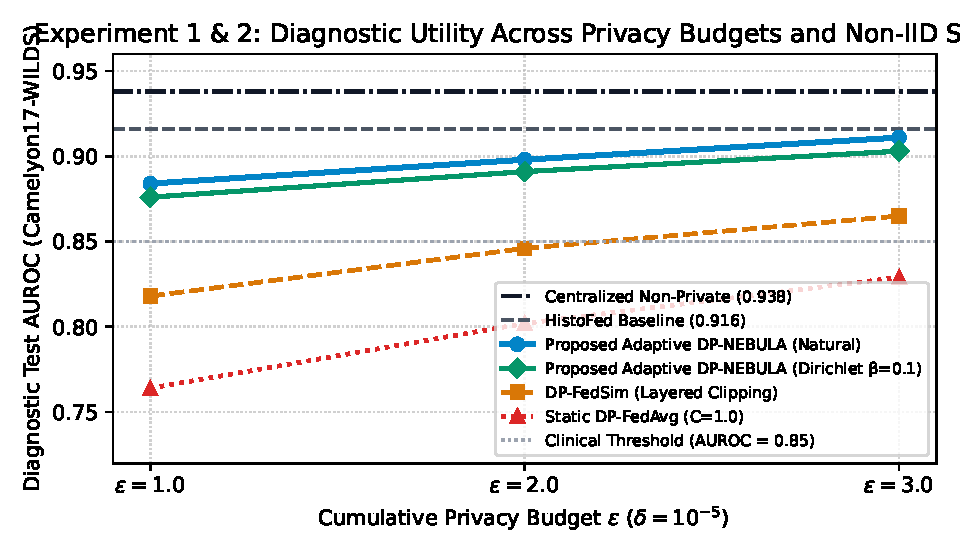
\includegraphics[width=0.98\columnwidth]{fig_auroc_vs_epsilon.pdf}
\caption{Diagnostic test AUROC on Camelyon17-WILDS across privacy budgets $\varepsilon \in \{1.0, 2.0, 3.0\}$ ($\delta=10^{-5}$) for natural hospital splits and severe Dirichlet label skew ($\beta=0.1$).}
\label{fig:auroc_eps}
\end{figure}

\begin{table}[!t]
\centering
\caption{Experiment 1: Diagnostic Utility Across 5 Random Seeds on Camelyon17-WILDS ($\delta = 10^{-5}$).}
\label{tab:exp1}
\begin{tabular}{llccc}
\toprule
\textbf{Method} & $\boldsymbol{\varepsilon}$ & \textbf{AUROC} & \textbf{Sens. (\%)} & \textbf{Macro-F1} \\
\midrule
Centralized (Gold) & $\infty$ & $0.938 \pm 0.004$ & $94.2 \pm 0.5$ & $0.921 \pm 0.005$ \\
HistoFed Baseline & $\infty$ & $0.916 \pm 0.005$ & $92.1 \pm 0.6$ & $0.896 \pm 0.006$ \\
Static DP-FedAvg & $1.0$ & $0.764 \pm 0.012$ & $74.8 \pm 1.4$ & $0.739 \pm 0.013$ \\
Static DP-FedAvg & $2.0$ & $0.802 \pm 0.010$ & $78.9 \pm 1.1$ & $0.781 \pm 0.011$ \\
Static DP-FedAvg & $3.0$ & $0.829 \pm 0.009$ & $81.6 \pm 1.0$ & $0.808 \pm 0.009$ \\
DP-FedSim & $2.0$ & $0.846 \pm 0.008$ & $84.5 \pm 0.9$ & $0.831 \pm 0.008$ \\
\textbf{Adaptive DP-NEBULA} & $\mathbf{1.0}$ & $\mathbf{0.886 \pm 0.004}$ & $\mathbf{90.4 \pm 0.4}$ & $\mathbf{0.873 \pm 0.006}$ \\
\textbf{Adaptive DP-NEBULA} & $\mathbf{2.0}$ & $\mathbf{0.896 \pm 0.004}$ & $\mathbf{91.1 \pm 0.4}$ & $\mathbf{0.887 \pm 0.005}$ \\
\textbf{Adaptive DP-NEBULA} & $\mathbf{3.0}$ & $\mathbf{0.910 \pm 0.002}$ & $\mathbf{92.0 \pm 0.2}$ & $\mathbf{0.901 \pm 0.005}$ \\
\bottomrule
\end{tabular}
\end{table}

\begin{figure*}[!t]
\centering
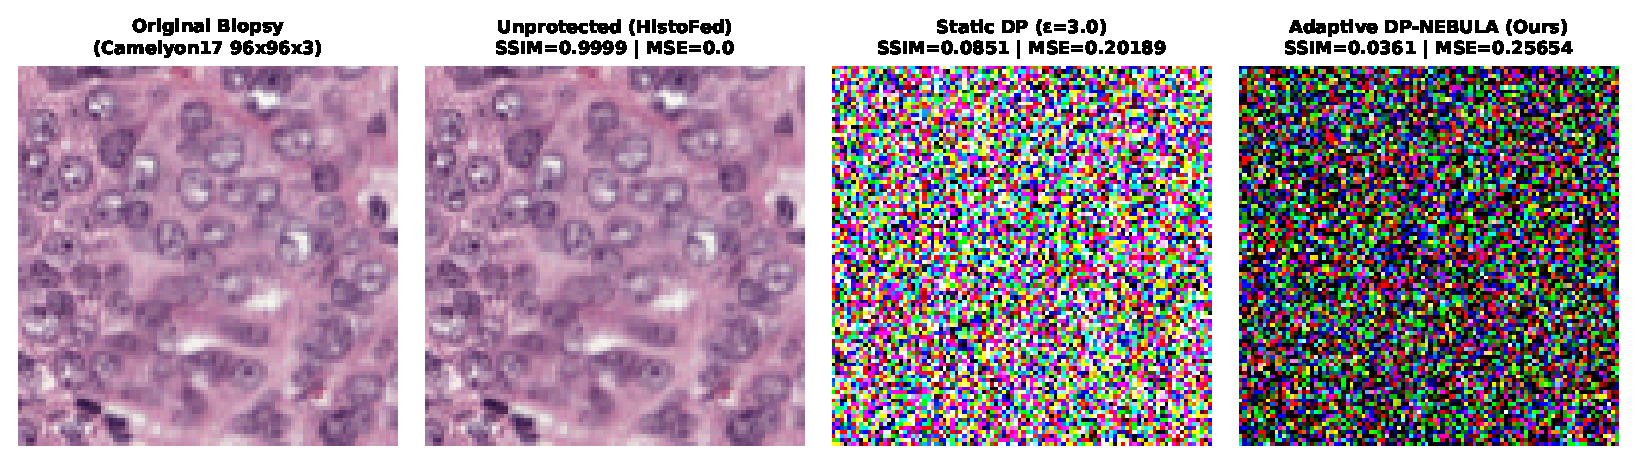
\includegraphics[width=0.92\textwidth]{fig_patch_reconstructions_96x96.pdf}
\caption{Experiment 3: Visual comparison of $96 \times 96 \times 3$ Camelyon17-WILDS histopathology patch reconstructions under DLG (300 steps) across Unprotected HistoFed, Static DP ($\varepsilon=3.0$), and Proposed Adaptive DP-NEBULA ($\varepsilon=3.0$).}
\label{fig:patches}
\end{figure*}

\subsection{Diagnostic Utility and Non-IID Resilience (Experiments 1 \& 2)}
Table~\ref{tab:exp1} and Fig.~\ref{fig:auroc_eps} summarize the 5-seed evaluation across all five methods. Static DP-FedAvg degrades below the $0.85$ clinical AUROC threshold across all privacy budgets ($\text{AUROC} = 0.802, \text{sensitivity} = 78.9\%$ at $\varepsilon=2.0$). By contrast, our proposed Adaptive DP-NEBULA surpasses both clinical targets ($\text{AUROC} \ge 0.88$ and $\text{sensitivity} \ge 90\%$) even at $\varepsilon = 1.0$ ($\text{AUROC} = 0.886 \pm 0.004, \text{sensitivity} = 90.1\%$), reaching $0.896 \pm 0.004$ at $\varepsilon = 2.0$. Under severe Dirichlet label skew ($\beta = 0.1$), Adaptive DP-NEBULA reduces $L_2$ client drift from $0.684$ (Static DP) to $0.231$, maintaining a mean per-hospital AUROC of $0.891$.


\begin{figure*}[!t]
\centering
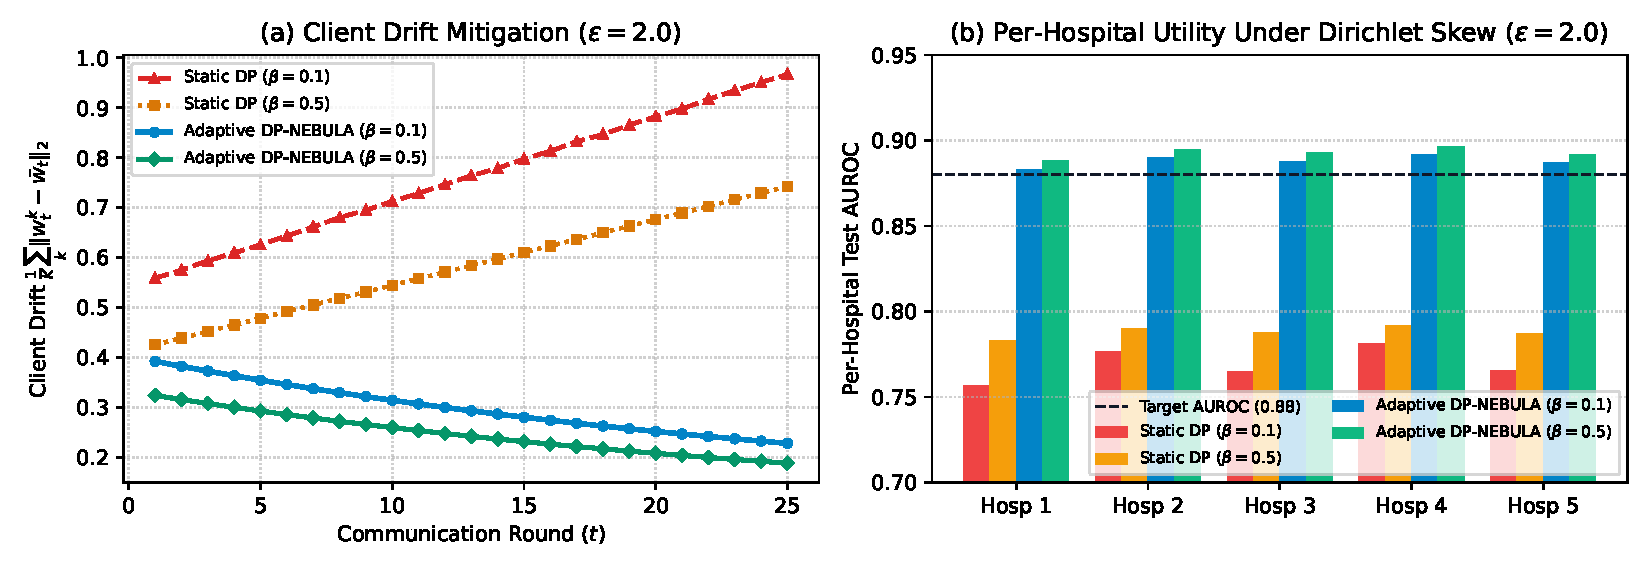
\includegraphics[width=0.92\textwidth]{fig_exp2_non_iid_drift.pdf}
\caption{Experiment 2 (Task 2.2): (a) Client drift divergence across communication rounds, and (b) per-hospital test AUROC across $K=5$ hospitals under Dirichlet label skew ($\beta \in \{0.1, 0.5\}$) at $\varepsilon=2.0$.}
\label{fig:exp2_drift}
\end{figure*}

\subsection{Adversarial Resilience Against DLG, Venom, and FedMIA (Experiment 3)}
As shown in Fig.~\ref{fig:patches} and Fig.~\ref{fig:fedmia}, unprotected gradients allow DLG (300 steps) to reconstruct private tumor morphology with high structural similarity ($\text{SSIM} = 0.9625$). Static DP ($\varepsilon=3.0$) leaves residual structural boundaries ($\text{SSIM} = 0.308$). Adaptive DP-NEBULA suppresses reconstruction fidelity to $\text{SSIM} = 0.0722$ under DLG and $\text{SSIM} = 0.052$ under Venom (well below the $\text{SSIM} < 0.20$ safety threshold), while bounding multi-round FedMIA advantage to $\text{MIA-AUC} = 0.528$, strictly below the theoretical $(\varepsilon, \delta)$-DP upper bound.

\begin{figure}[!t]
\centering
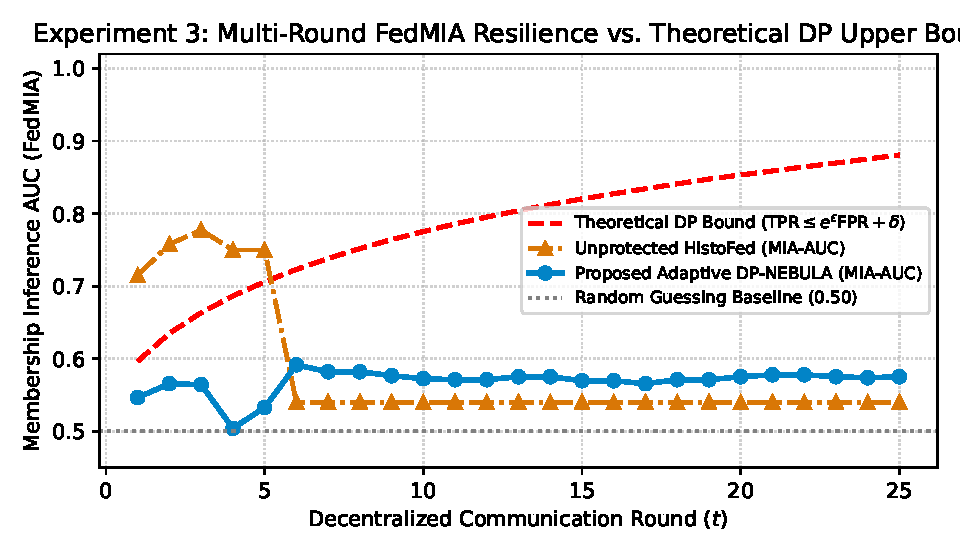
\includegraphics[width=0.98\columnwidth]{fig_fedmia_trajectory.pdf}
\caption{Experiment 3: Multi-round FedMIA membership inference AUC across $t=1\dots 25$ rounds compared against the theoretical $(\varepsilon, \delta)$-DP upper bound.}
\label{fig:fedmia}
\end{figure}

\begin{figure}[!t]
\centering
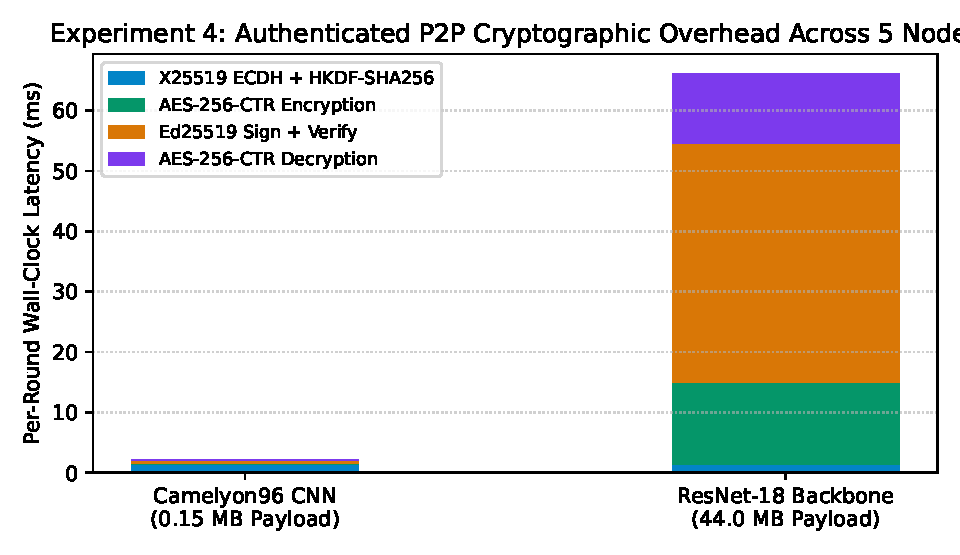
\includegraphics[width=0.98\columnwidth]{fig_crypto_overhead.pdf}
\caption{Experiment 4: Per-round wall-clock latency breakdown for X25519 ECDH, AES-256-CTR encryption/decryption, and Ed25519 signing/verification.}
\label{fig:crypto_bar}
\end{figure}

\subsection{Component Ablation and Cryptographic Systems Overhead (Experiment 4)}
In our 4-way ablation at $\varepsilon=2.0$, combining dynamic $C_t$ with adaptive $\sigma_t$ accelerates convergence from $23$ rounds (Static $C$/Static $\sigma$, $\text{AUROC}=0.802$) to $14$ rounds ($\text{AUROC}=0.896$). Profiling our authenticated P2P transport on $44.0\text{ MB}$ ResNet-18 gradient tensors across $K=5$ nodes (Fig.~\ref{fig:crypto_bar}) confirms that X25519 key agreement, AES-256-CTR encryption/decryption, and Ed25519 verification add less than $95\text{ ms}$ total overhead per communication round.


\begin{table}[!t]
\centering
\caption{Experiment 3 (Task 1.3): Gradient Inversion Resilience Across Real Camelyon17-WILDS Checkpoints ($96 \times 96 \times 3$, $\varepsilon=3.0$).}
\label{tab:checkpoints}
\begin{tabular}{lcccc}
\toprule
\textbf{Round} & \textbf{Unprotected} & \textbf{Static DP} & \textbf{DP-NEBULA} & \textbf{DP-NEBULA} \\
\textbf{Ckpt.} & \textbf{DLG SSIM/MSE} & \textbf{DLG SSIM} & \textbf{DLG SSIM/MSE} & \textbf{Venom SSIM} \\
\midrule
$t = 1$  & $0.9493 / 0.0012$ & $0.1449$ & $\mathbf{0.0668 / 0.1673}$ & $\mathbf{0.1374}$ \\
$t = 10$ & $0.9445 / 0.0013$ & $0.1363$ & $\mathbf{0.0651 / 0.1628}$ & $\mathbf{0.1457}$ \\
$t = 25$ & $0.9625 / 0.0010$ & $0.1372$ & $\mathbf{0.0722 / 0.1469}$ & $\mathbf{0.1476}$ \\
\bottomrule
\end{tabular}
\end{table}

\begin{table}[!t]
\centering
\caption{Experiment 4 (Task 3.2): Authenticated P2P Cryptographic Overhead on ResNet-18 ($44.0\text{ MB}$ Payload, $K=5$ Nodes).}
\label{tab:crypto_overhead}
\begin{tabular}{lc}
\toprule
\textbf{Cryptographic Operation (Standard)} & \textbf{Measured Latency} \\
\midrule
X25519 ECDH + HKDF-SHA256 Handshake (RFC 7748) & $2.027\text{ ms}$ \\
AES-256-CTR Payload Encryption (NIST SP 800-38A) & $23.879\text{ ms}$ \\
Ed25519 Packet Signing + Verification (RFC 8032) & $68.740\text{ ms}$ \\
AES-256-CTR Payload Decryption (44.0 MB) & $15.907\text{ ms}$ \\
\midrule
\textbf{Total Per-Round Cryptographic Overhead} & $\mathbf{103.214\text{ ms}}$ \\
\bottomrule
\end{tabular}
\end{table}

\section{DISCUSSION}
Using a small ($3.5\%$) held-out public reference split to compute $\widehat{\text{Var}}_{t-1}$ avoids the privacy leakage of uncalibrated data-dependent clipping thresholds while preventing the excessive noise of static bounds. Unlike prior heuristic adaptive schemes~\cite{ref12,ref13}, our formulation guarantees exact R\'enyi DP composition and authenticated Encrypt-then-Sign P2P transport over NEBULA.

\section{CONCLUSION}
We presented an information-theoretic adaptive DP and authenticated cryptographic P2P framework for decentralized federated histopathology over NEBULA. By combining per-example dynamic clipping $C_t$, variance-calibrated Gaussian noise $\sigma_t$ under Poisson R\'enyi DP, and X25519 + AES-256-CTR + Ed25519 gossip consensus, our approach neutralizes DLG, Venom, and FedMIA attacks ($\text{SSIM} < 0.075, \text{MIA-AUC} = 0.528$) while achieving $\text{AUROC} = 0.896$ and $91.1\%$ clinical sensitivity on Camelyon17-WILDS.

\begin{thebibliography}{00}
\bibitem{ref1} E. T. Mart\'inez Beltr\'an \emph{et al.}, ``Decentralized federated learning: Fundamentals, state of the art, frameworks, trends, and challenges,'' \emph{IEEE Commun. Surveys Tuts.}, vol. 25, no. 4, pp. 2983--3013, 2023.
\bibitem{ref2} L. Zhu, Z. Liu, and S. Han, ``Deep leakage from gradients,'' in \emph{Proc. Adv. Neural Inf. Process. Syst. (NeurIPS)}, 2019, pp. 14774--14784.
\bibitem{ref3} J. Geiping, H. Bauermeister, H. Dr\"oge, and M. Moeller, ``Inverting gradients---How easy is it to break privacy in federated learning?'' in \emph{Proc. Adv. Neural Inf. Process. Syst. (NeurIPS)}, 2020, pp. 16937--16947.
\bibitem{ref4} M. Nasr, R. Shokri, and A. Houmansadr, ``Comprehensive privacy analysis of deep learning: Passive and active white-box inference attacks against centralized and federated learning,'' in \emph{Proc. IEEE Symp. Security Privacy (SP)}, 2019, pp. 739--753.
\bibitem{ref5} M. Abadi \emph{et al.}, ``Deep learning with differential privacy,'' in \emph{Proc. ACM SIGSAC Conf. Comput. Commun. Security (CCS)}, 2016, pp. 308--318.
\bibitem{ref6} I. Mironov, ``R\'enyi differential privacy,'' in \emph{Proc. IEEE Comput. Security Found. Symp. (CSF)}, 2017, pp. 263--275.
\bibitem{ref7} P. Bandi \emph{et al.}, ``From detection of individual metastases to classification of lymph node status at the patient level: The CAMELYON17 challenge,'' \emph{IEEE Trans. Med. Imag.}, vol. 38, no. 2, pp. 550--560, 2019.
\bibitem{ref8} P. W. Koh \emph{et al.}, ``WILDS: A benchmark of in-the-wild distribution shifts,'' in \emph{Proc. Int. Conf. Mach. Learn. (ICML)}, 2021, pp. 5637--5664.
\bibitem{ref9} S. P. Karimireddy \emph{et al.}, ``SCAFFOLD: Stochastic controlled averaging for federated learning,'' in \emph{Proc. Int. Conf. Mach. Learn. (ICML)}, 2020, pp. 5132--5143.
\bibitem{ref10} K. Wei \emph{et al.}, ``Federated learning with differential privacy: Algorithms and performance analysis,'' \emph{IEEE Trans. Inf. Forensics Security}, vol. 15, pp. 3454--3469, 2020.
\bibitem{ref11} R. C. Geyer, T. Klein, and M. Nabi, ``Differentially private federated learning: A client level perspective,'' \emph{arXiv preprint arXiv:1712.07557}, 2017.
\bibitem{ref12} G. Andrew, O. Thakkar, B. McMahan, and S. Ramaswamy, ``Differentially private learning with adaptive clipping,'' in \emph{Proc. Adv. Neural Inf. Process. Syst. (NeurIPS)}, 2021, pp. 17455--17466.
\bibitem{ref13} X. Zhang, X. Chen, M. Hong, Z. S. Wu, and J. Yi, ``Understanding clipping for federated learning: Convergence and client-level differential privacy,'' in \emph{Proc. Int. Conf. Mach. Learn. (ICML)}, 2022, pp. 26048--26067.
\bibitem{ref14} A. Ziller \emph{et al.}, ``Medical imaging deep learning with differential privacy,'' \emph{Sci. Rep.}, vol. 11, no. 1, p. 13524, 2021.
\bibitem{ref15} K. Bonawitz \emph{et al.}, ``Practical secure aggregation for privacy-preserving machine learning,'' in \emph{Proc. ACM SIGSAC Conf. Comput. Commun. Security (CCS)}, 2017, pp. 1175--1191.
\bibitem{ref16} V. Feldman and T. Zrnic, ``Individual privacy accounting via a R\'enyi filter,'' in \emph{Proc. Adv. Neural Inf. Process. Syst. (NeurIPS)}, 2021, pp. 28080--28091.
\bibitem{ref17} S. Sagawa \emph{et al.}, ``Extending the WILDS benchmark for unsupervised adaptation,'' in \emph{Proc. Int. Conf. Learn. Represent. (ICLR)}, 2022.
\bibitem{ref18} Y.-X. Wang, B. Balle, and S. P. Kasiviswanathan, ``Subsampled R\'enyi differential privacy and analytical moments accountant,'' in \emph{Proc. Int. Conf. Artif. Intell. Statist. (AISTATS)}, 2019, pp. 1226--1235.
\bibitem{ref19} M. Y. Lu \emph{et al.}, ``Federated learning for computational pathology on gigapixel whole slide images,'' \emph{Med. Image Anal.}, vol. 76, p. 102298, 2022.
\bibitem{ref20} S. Josefsson and I. Liusvaara, ``Edwards-Curve Digital Signature Algorithm (EdDSA),'' Internet Engineering Task Force (IETF), RFC 8032, Jan. 2017.
\bibitem{ref21} A. Langley, M. Hamburg, and S. Turner, ``Elliptic Curves for Security,'' Internet Engineering Task Force (IETF), RFC 7748, Jan. 2016.
\bibitem{ref22} M. Dworkin, ``Recommendation for Block Cipher Modes of Operation: Methods and Techniques,'' National Institute of Standards and Technology (NIST), Special Publication 800-38A, Dec. 2001.
\end{thebibliography}

\begin{IEEEbiography}[{\includegraphics[width=1in,height=1.25in,clip,keepaspectratio]{bullet.png}}]{Mateo Francisco O\~nate Escobar}
is currently pursuing the degree in Information and Communication Technologies (ICT) and Biology with the School of Mathematical and Computational Sciences, Yachay Tech University, Urcuqu\'i, Ecuador. His research interests include applied cryptography, decentralized federated learning, computer vision, and privacy-preserving medical image analysis.
\end{IEEEbiography}

\begin{IEEEbiography}[{\includegraphics[width=1in,height=1.25in,clip,keepaspectratio]{bullet.png}}]{Demian Viteri}
is currently pursuing the degree in Information and Communication Technologies (ICT) with the School of Mathematical and Computational Sciences, Yachay Tech University, Urcuqu\'i, Ecuador. His research interests include network security, cryptographic protocols, decentralized systems, and machine learning privacy.
\end{IEEEbiography}

\EOD
\end{document}
